\chapter{Voorgestelde testmethodiek }	\label{sec:methodiekvantesten}
Dit hoofdstuk behandelt de wijze waarop de testen naar consistentie en beschikbaarheid worden uitgevoerd. 
De methodiek is opgedeeld in 4 grote stappen: het opstellen, kalibreren, testen van de systemen en tenslotte het verzamelen en analyseren van de resultaten. Een overzicht van de procedure kan gevonden worden in figuur \ref{fig:test-process-overview}.

\paragraph{Opstellen van de testomgeving} Deze eerste stap is voor het selecteren, installeren en configureren van een DBMS en de testsoftware. Een variatie in hardware van de systemen, versienummer van de software of een verschillende netwerkinfrastructuur kan de uiteindelijke testresultaten beïnvloeden. 

\paragraph{Calibratie van de testomgeving} In de uiteindelijke testen wordt het gedrag onder matige belasting getest. Afhankelijk van de gekozen systemen, netwerkinfrastructuur zal dit voor elke DBMS een verschillende belasting geven. Deze stap bepaalt welke queries er uitgevoerd worden, hoeveel gebruikers er zijn in het systeem en hoeveel bewerkingen er uitgevoerd worden per second. 

\paragraph{Testen van de systemen} In deze stap worden de testen op de verschillende systemen uitgevoerd. Deze methodiek maakt het mogelijk om te testen hoe de vertraging op een bewerken zich gedraagt voor, tijdens en na het falen en herstellen van een systeem. Voor de consistentie wordt het mogelijk om zowel aan passieve als actieve analyse te doen. 

\paragraph{Verzamelen en analyseren van de testdata} In de laatste stap wordt de data van de vorige stappen verzameld en de resultaten worden visueel voorgesteld. Met behulp van de uitgebreide testdata, is het ook mogelijk om bepaalde conclusies te maken over een de beschikbaarheids- en consistentiegaranties van de verschillende. 

In de volgende secties komen de verschillende stappen in meer detail aan bod.  
\begin{figure}[ht!]
\centering
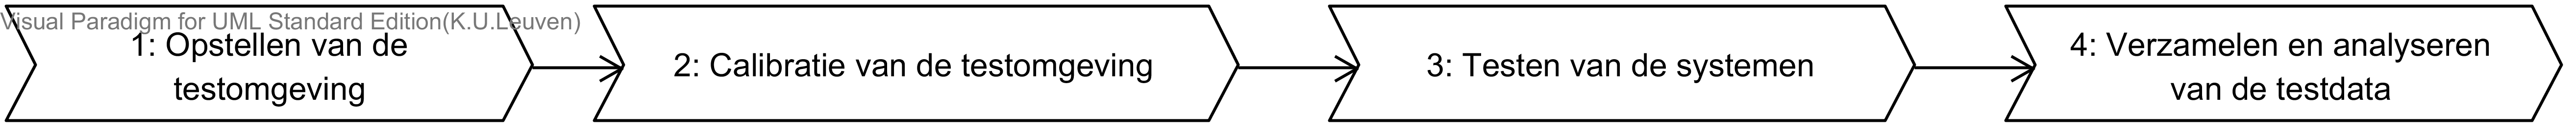
\includegraphics[width=\linewidth]{img/Test-Process-Overview}
\caption{Overzicht testproces}
\label{fig:test-process-overview}
\end{figure}

\section{Stap 1: Opstellen van de testomgeving}
\paragraph{Keuze van DBMS's} In eerste instantie moet er gekozen worden welke DBMS's er getest worden. Er zijn verschillende mogelijke keuzes, er kan een enkele systeem getest worden in één of meerdere configuraties of verschillende systemen. 

\paragraph{Bepalen van de infrastructuur}Na van de systemen kan de configuratie van de testomgeving gebeuren. Dit gebeurt eerst door het aantal instanties per systeem te beslissen en de hardware te kiezen. 

\paragraph{Installatie en configuratie} Het lokaal installeren en configureren een softwarepakket, is in Unix veelvuldig geautomatiseerd met behulp van tools zoals \textit{apt-get} en \textit{yum}. Voor een systeem in een gedistribueerde omgeving, is de situatie ingewikkelder. In een gedistribueerd systeem, dienen de verschillende servers van elkaar op de hoogte gebracht.

In een gedistribueerde configuratie stap worden de verschillende systemen van elkaars bestaan op de hoogte gebracht en worden de relaties opgezet. Hiervoor bestaan er twee verschillende methodes maar ook een combinatie is mogelijk.
 
\subparagraph{Configuratie bestanden} Met deze methode heeft elke lokaal systeem een configuratiebestand met hierin een link naar één of meerdere andere instanties. Nadat de administrator deze configuratie heeft aangemaakt, kan het DBMS gestart worden. Deze informatie kan een ip adres of de hostname zijn waarbij soms 1 instantie voldoende is, bij andere moeten ze allemaal opgegeven worden. 
\subparagraph{Centrale configuratie} Bij een centrale configuratie, worden de systemen lokaal opgestart zonder informatie van de andere instanties. Vervolgens wordt via een console, webinterface, ... connectie gemaakt met een node. Deze krijgt configuratie informatie hoe deze zich moet gedragen en volgt deze informatie op. In deze systemen is de configuratie tijdens installatie gelijk en wordt de configuratie verspreid wanneer de systemen al draaien.  

Na het uitvoeren van deze stap, zou het DBMS moeten werken zoals vereist. 

\section{Stap 2: Calibratie van de testomgeving}
Afhankelijk van de onderliggende infrastructuur en het soort DBMS, kan het systeem een verschillend gedrag hebben onder dezelfde configuratie. Voor de eigenlijk testen is het de bedoeling om een middelmatige belasting te hebben. De queueing theorie geeft de eigenschap dat de totale vertraging (R) gelijk is aan de som van verwerkings- (S) en wachttijd (W)\cite{millsap2003optimizing}. Dit verband is visueel voorgesteld ten opzichte van de belasting in figuur \ref{fig:hockey-stick}. 

\begin{figure}[ht!] 
\centering
	\subfigure[Verband vertraging ten opzicht van de belasting van een DBMS.]{\label{fig:hockey-stick} 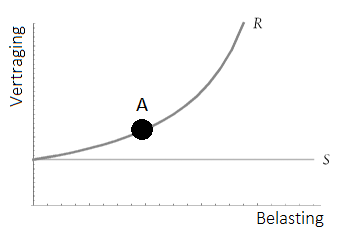
\includegraphics[width=0.45\textwidth]{img/hockey-stick}}
	\hfill
	\subfigure[Verband aantal requests/seconde ten opzicht van het aantal gebruikers.]{\label{fig:connecties-gebruikers} 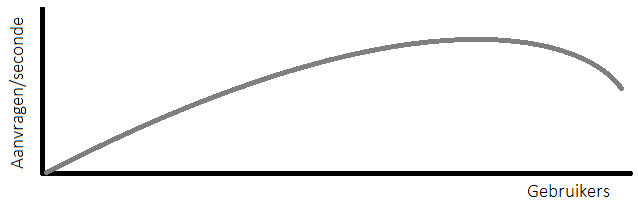
\includegraphics[width=0.45\textwidth]{img/connecties-gebruikers}}
	\caption{Verbanden voor de calibratie}
\end{figure}
Deze belasting kan afhankelijk zijn verschillende elementen, er worden 5 verschillende mogelijke parameter groepen besproken:

\paragraph{Hoeveelheid data per gegevensrecord} Elke record in de database kan bestaan uit verschillende kolommen en per kolom een waarde. Het is belangrijk om te definiëren hoe groot een gemiddeld record is, het type data in een record en het aantal kolommen. Een klein record zorgt voor minder netwerkverkeer en een ander schrijfgebruik dan bij een groot record. 

\paragraph{Type van queries} De opgeslagen data kan opgevraagd worden op verschillende wijze. Data kan ingevoegd, aangepast, opgevraagd of verwijderd worden. Daarnaast kan dit gebeuren voor 1 of meerdere records tegelijk. Afhankelijk van de relatieve verhouding van deze soorten, kan een ander resultaat bekomen worden: sommige DBMS's zijn meer geschikt voor een dominantie in leesacties andere voor schrijfacties. Enkele systemen lezen data goed in grote hoeveelheid, andere lezen zeer goed in kleine hoeveelheden. 

\paragraph{Query specificatie} Bij het opvragen of verwijderen van een record, kan er een verschil zijn naar processing tijd afhankelijk van hoe lang geleden de record geschreven of gelezen is en of naburige data onlangs gelezen is. Vandaar dat ook het datadistributie gekozen moet worden. Voorbeelden van verschillende technieken zijn: voornamelijk de laatste data lezen, een uniforme kans voor alle data of bepaalde records regelmatig lezen.

\paragraph{Aantal connecties of gebruikers} Een gedistribueerde omgeving heeft meestal meerdere gebruikers die tegelijk actief zijn. Maar sommige systemen hebben een voorkeur naar weinig connecties met grote hoeveelheden data, andere kunnen meer gebruikers tegelijk behandelen. Het totaal aantal queries kan berekend worden als: $\#Queries = \#Gebruikers * \#QueriesPerGebruiker$. In deze stap wordt er verondersteld dat de gebruiker het maximaal aantal queries doet, dus $1/Vertraging$. Rekening houdend met de exponentiële groei van de wachtrij vertraging (figuur \ref{fig:hockey-stick}), betekent dit dat er een maximum aantal queries per seconde bereikt wordt bij een bepaald aantal gebruikers. In deze stap wordt er gezocht naar dit aantal gebruikers. De grafiek zal er meestal uitzien zoals in figuur \ref{fig:connecties-gebruikers}. 

\paragraph{Aantal queries per seconde} In de vorige stap is er de optimale configuratie bepaald om het systeem maximaal te belasten. In het begin is er gesteld dat er gezocht wordt naar een gemiddelde belasting voor dit aantal gebruikers. Er wordt gekozen om matige belasting, in figuur \ref{fig:hockey-stick} zou dit punt A zijn. 

Met de parameters afkomstig uit de calibratie, kunnen de testen opgestart en uitgevoerd worden. 

\section{Stap 3: Testen van de systemen} \label{sec:testenvandesystemen}
In deze thesis zullen er 2 verschillende soort testen uitgevoerd worden, de beschikbaarheid en consistentietesten, welke dezelfde algemene stappen volgen, elk met hun eigen specifieke parameters. Er zijn de 6 deelstappen: 

\paragraph{Opstellen van de database} In stap 2 was er gekozen voor een bepaalde datastructuur. Deze structuur wordt zo goed mogelijk ingesteld in de DBMS zodat deze optimale allocatie kan doen.

\paragraph{Inladen van de data} Een bepaalde hoeveel data wordt vooraf ingeladen. Dit wordt gedaan om een basis hoeveelheid data te hebben die nodig is voor de initialisatie van de database. Zo wordt er met deze dataset sharding toepast, het opsplitsen van de data over verschillende servers. In bepaalde DBMS's wordt data automatisch opgesplitst bij het groeien van de dataset, om deze reden wordt er data ingeladen zodat deze automatische sharding gebeurt. Dit inladen van de data gebeurt op maximale snelheid. 

\paragraph{Pauze} Na het inladen van de data wordt enige tijd gewacht. Zoals aangetoond in YCSB++\cite[Figuur 9]{patil2011ycsb++}, is er hogere vertraging in de DBMS's onmiddellijk na het inlezen. Dit kan onder andere te wijten zijn doordat data nog weggeschreven moet worden naar schijf of in bepaalde systemen zou het kunnen dat de sharding gebeurt op momenten met weinig belasting. Met het toevoegen van de wachtperiode wordt de piek in de vertraging vermeden. 

\paragraph{Opstarten van de test (opstart kost)} De test wordt opgestart. In veel gevallen is er in het begin een opwarmfase nodig omdat de vertraging net hoger of lager is als na enige tijd. Deze hogere tijd is onder andere te verklaren door de connecties opgezet moet worden en caches voor gelezen data worden gevuld. Soms is deze lager omdat de schijf nog niet belast is of de er nog veel schrijfbuffers leeg zijn. Om dit gedrag te vermijden, wordt de data verzameld de eerste seconden niet gebruikt voor de analyse. 

\paragraph{Uitvoeren van de test} De eigenlijke test wordt uitgevoerd, de data wordt verzameld en opgeslagen. De details van de beide testen volgen achteraf. 

\paragraph{Terugbrengen naar beginstatus} Na het uitvoeren van de test, wordt het DBMS terug naar de beginstatus gebracht. Onder andere de database en de data wordt volledig verwijderd. Belangrijk in dit geval is het controleren of de data volledig verwijderd is, in bepaalde gevallen wordt er nog ergens een veiligheidskopie bijgehouden dat een volgende test kan beïnvloeden. 

De twee verschillende testmethodes zullen nu in meer detail behandeld worden. 
\subsection{Beschikbaarheidstest}
Bij de beschikbaarheidstest wordt er gekeken hoe het systeem reageert op tijdelijke, (on)verwachte onbeschikbaarheid van een deel van het systeem. In deze testen worden er 3 mogelijke manieren getest die de systemen onbeschikbaar maakt, terwijl er de belasting uit de calibratie wordt toegepast. 

\paragraph{Zachte stop} De DMBS service wordt gevraagd om te stoppen. Op deze manier krijgt de service eerst een signaal dat deze moet stoppen en kan deze de andere waarschuwen. Achteraf wordt dezelfde service terug opgestart. Dit simuleert het gepland uitschakelen van een systeem. 

\paragraph{Harde stop} De DMBS service wordt onmiddellijk gestopt door het process te beëindigen. De service heeft geen tijd om de andere te waarschuwen. Achteraf wordt dezelfde service terug opgestart. Dit simuleert een crash van de service die de systeembeheerders later opmerken en de service opnieuw opgestart wordt. 

\paragraph{Netwerk onderbreken} Al het in- en uitgaand netwerkverkeer wordt gestopt zonder enige waarschuwing. De service heeft geen tijd om de andere te waarschuwen én de zender krijgt geen onbereikbaar antwoord. Achteraf wordt het netwerk verkeer terug toegelaten. Dit simuleert een onderbroken internetverbinding of een gecrashte server.  

Eenzelfde systeem kan sterk verschillend reageren op de verschillende situaties: waar de eerste situatie nog eenvoudig is te behandelen doordat het systeem de andere op de hoogte kan brengen. In de tweede situatie wordt het moeilijker omdat het de andere systemen niet op de hoogte kunnen gebracht worden. Maar de systemen krijgen bij het contacteren het antwoord dat de service onbeschikbaar is. De derde situatie is het moeilijkste te behandelen omdat men niet weet of de berichten naar de server niet aankomen of de antwoorden verloren gaan. 

In dit geval kan er onderzoek gedaan worden naar het verschil in vertraging en de beschikbaarheid van de laatst geschreven data elementen. In dit onderzoek is er enkel gefocust op de reactie naar de vertraging toe. 
 
\subsection{Consistentietest}
In de consistentietest wordt onderzocht welke consistentie het DBMS ondersteund. Zoals voordien besproken in deel \ref{sec:eventualconsistency}, bestaan er verschillende soorten. 

In deze testen is er gekozen om caching bij de gebruiker \textbf{uit te schakelen}, dit om de reden dat dit gedrag zeer onvoorspelbaar is en afhankelijk van andere acties van de lezer en schrijver. Een andere reden is dat eventueel consistentie alleen een probleem is voor data die onmiddellijk beschikbaar moet zijn, met andere woorden data die men niet mag cachen. Dit heeft als gevolg dat de belasting op de server hoger kan zijn. 

\paragraph{Beschrijving van de test} Deze test bestaat uit 3 soorten gebruikers: er is een gebruiker die data schrijft (=S), een aantal lezer (=L's) en tenslotte zijn er nog andere gebruikers die zorgen voor de basisbelasting. De berekening van deze basisbelasting komt verder aanbod.  
Het is belangrijk dat er een exacte synchronisatie in tijd is tussen de verschillende gebruikers, dit om de geregistreerde tijdstippen te kunnen vergelijken.


\subparagraph{Taak van de schrijver} De schrijver schrijft, zoals zijn naam voorspelt, voorafbepaalde data weg op vooraf vastgelegde momenten. De data kan een nieuw record of een update van een record zijn. De schrijver registreert op welk exact tijdstip deze taak is gestart, hoe en wanneer deze is beëindigd.

\subparagraph{Taak van de lezer} De taak van een individuele lezer is om op vooraf vastgelegde momenten de data van de schrijven te gaan lezen. Dit wordt periodiek herhaald tot de data correct is gelezen of een bepaalde tijd is verstreken. Er kan ook beslist worden om ook als de data correct gelezen is, te blijven lezen om te zien of het resultaat terug veranderd. De lezer registreert elke keer deze gaat lezen op welk moment deze exact is gaan lezen en wat het resultaat van de actie is.  

\subparagraph{Het plannen van de lezers} Het doel van de verschillende lezers is om allereerst verbonden te zijn met verschillende servers zoals ook gebruikers zullen zijn. Daarnaast zijn er  meer testpogingen voor het lezen van de data omdat verschillende lezers in parallel kunnen lezen. Om deze laatste redenen worden de starttijdstippen voor de data te lezen, gelijk gespreid tussen de verschillende lezers. Een voorbeeldperiode met 1 schrijver en 4 lezers kan gevonden worden in figuur \ref{fig:test-consistentietest-periode}. 

\begin{figure}[ht!]
\centering
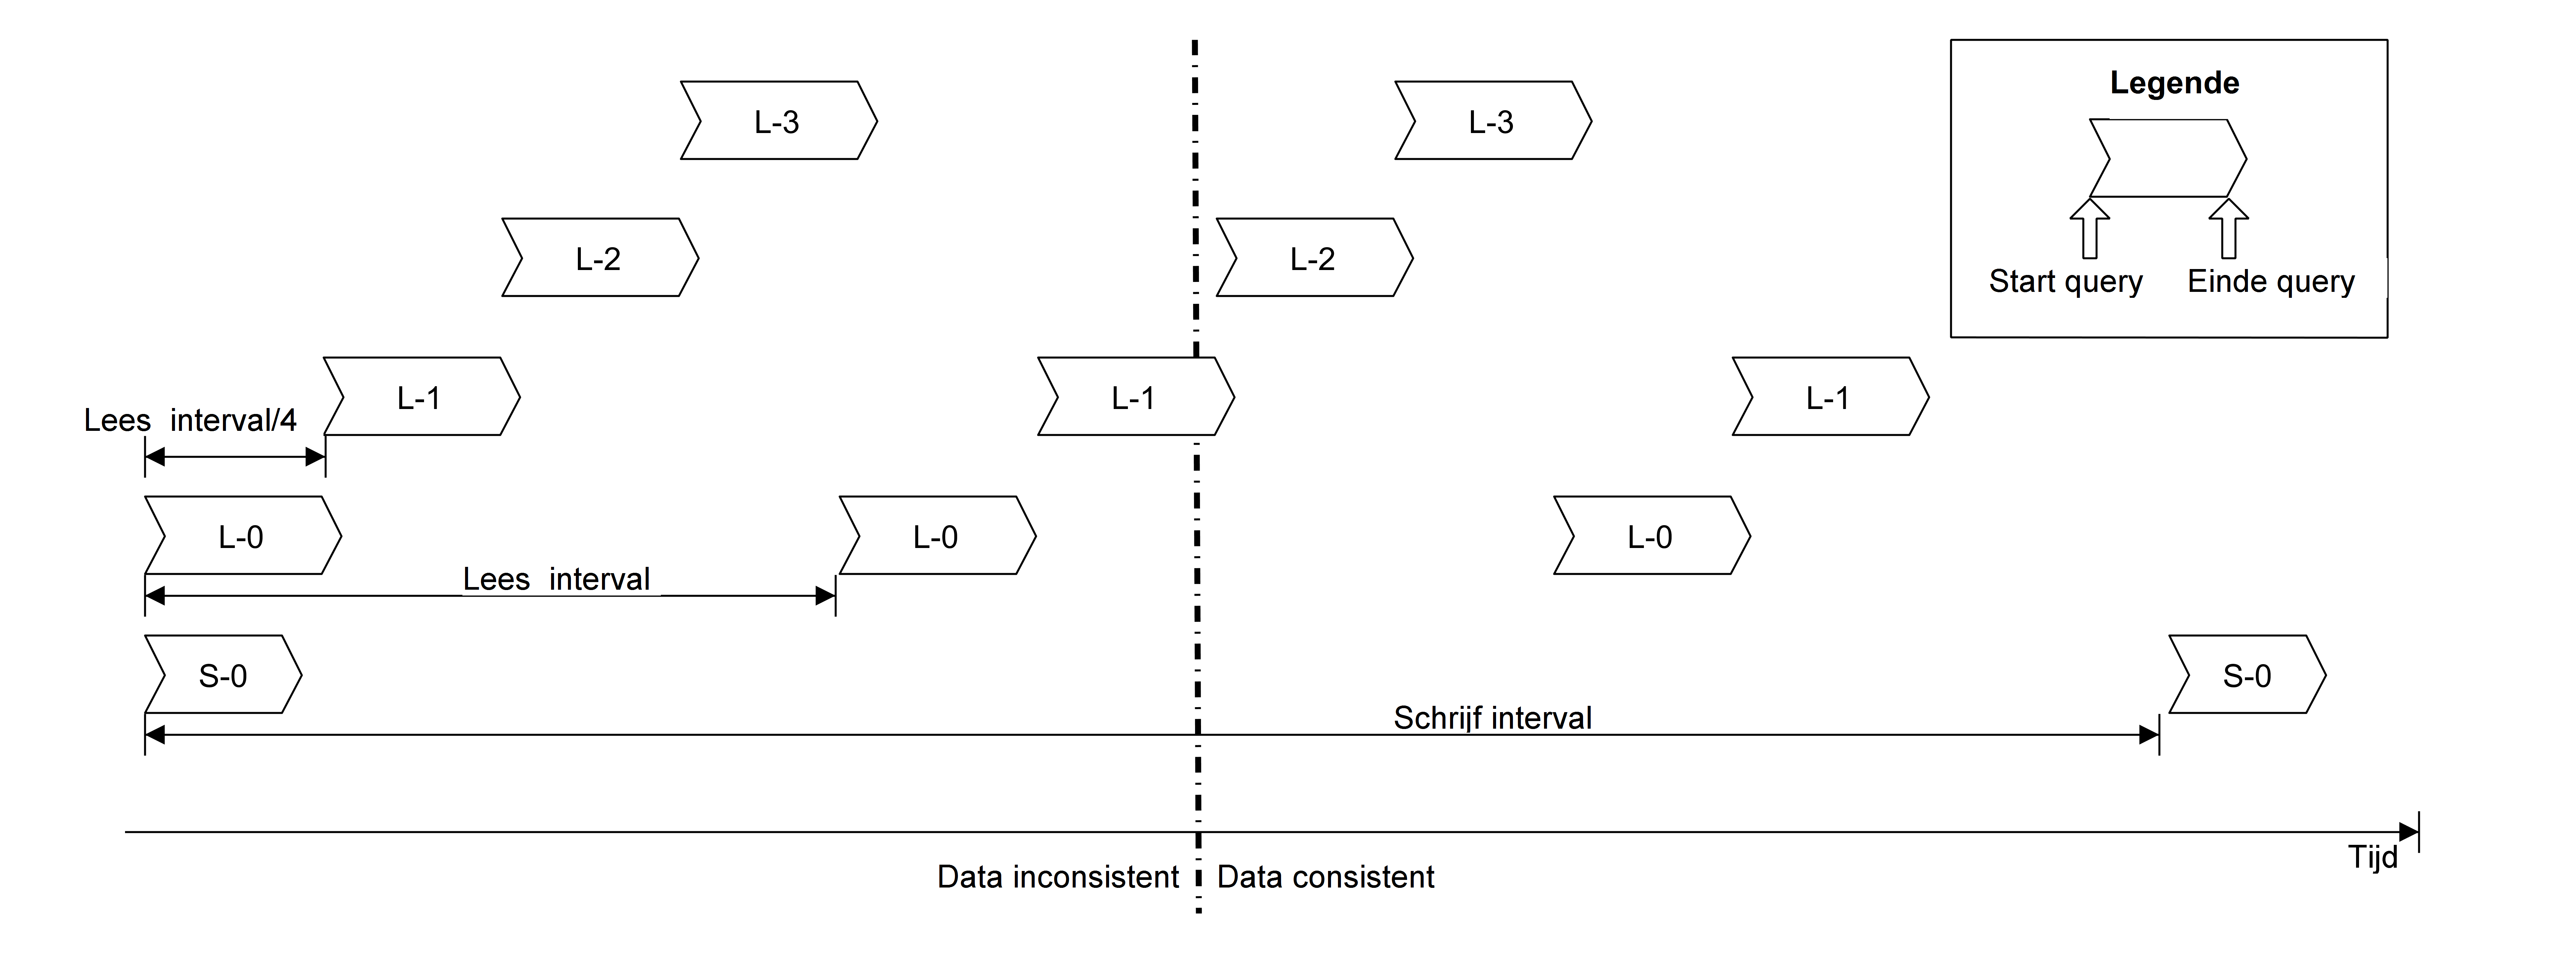
\includegraphics[width=\linewidth]{img/Consistentie-test-periode}
\caption{Consistentietest: Een enkele periode van de consistentietesten. Er is 1 schrijver, 4 lezers. De lezers stoppen zodra deze de data correct hebben gelezen. De rode lijn geeft aan vanaf wanneer de data consistent is voor alle queries gestart na dit tijdstip. }
\label{fig:test-consistentietest-periode}
\end{figure}


\subparagraph{Schatten van de basisbelasting} De basisbelasting kan de berekende belasting zijn in stap 2, waardoor het reëel aantal queries hoger ligt. De belasting kan ook verminderd worden met een geschat aantal queries die de schrijvers en lezers zullen uitvoeren. Het aantal queries van de schrijver en lezers per seconde kan berekend worden aan de hand van de hand van volgende formule: $(S + \#L*\#queriesperschrijfperiode / schrijfinterval$. Het aantal leesbewerkingen per schrijf periode zal geschat moeten worden, maar kan bijvoorbeeld op 1 gezet worden. Op deze manier krijgen systemen die geen strikte consistentie afdwingen een hogere belasting om de correcte waarde te lezen. Er zal immers een tweede keer of meer geprobeerd moeten worden. 

\paragraph{Soorten eventuele consistentie} Met deze uitgevoerde testen en data kan aangetoond worden dat bepaalde systemen bepaalde eventuele consistentie vereisten niet volgen. Het is in mogelijk om met deze testen een tegenvoorbeeld te vinden zie tonen dat een systeem een eigenschap niet garandeert. Maar het vinden van geen tegenvoorbeeld is geen bewijs, maar kan wel een indicatie zijn hoe vaak het kan voorkomen. 

\subparagraph{Consistentie} Een systeem is niet consistent indien één van de lezers het nieuwe record of de update niet leest \textit{indien de leesactie gestart is na het voltooien van de schrijfactie}. Als dit voorkomt, gedraagt het systeem zich niet alsof er maar een enkele data-instantie is. 

\subparagraph{Read your own writes consistentie} Deze eventuele consistentie kan ontkracht worden indien een schrijver onmiddellijk na het voltooien zijn eigen data opvraagt en niet de nieuwe waarde leest. Voor deze testen dient de server ondersteuning te bieden om meerdere connecties te hebben per gebruiker. 

\subparagraph{Session consistentie} Session consistentie is een verzwakking van de vorig eis. Het is nu slechts nodig om de data te lezen van een schrijfactie in een zelfde sessie, niet voor nieuwe sessies van dezelfde gebruiker. Dit kan ontkracht worden door met dezelfde connectie als de schrijver te lezen en de oude data te lezen. 

\subparagraph{Casual consistentie} Deze test kan uitgevoerd worden indien de schrijver verschillende schrijfacties na elkaar te laten uitvoeren. De lezer leest de records in dezelfde of omgekeerde volgorde. Indien deze data van een latere schrijfactie leest maar nog niet van een vroegere, is dit ongeldig. De eis kan strenger gemaakt worden door de schrijver tussendoor niet te laten lezen, dit zou andere resultaten kunnen hebben. Deze consistentie is niet getest. 

\subparagraph{Monotonic Read consistentie} In deze test blijft de lezer continue opnieuw proberen om dezelfde data te lezen. Eenmaal deze een nieuwe versie heeft gelezen, zou deze nooit meer oudere data mogen lezen. 

Zoals duidelijk hierboven, biedt deze aanpak de mogelijkheid aan om naast een actieve ook een passieve analyse te doen op de data. In deze thesis zal er gefocust worden op de \textit{read your own writes} en \textit{monotonic read} consistentie. 

\section{Stap 4: Verzamelen en analyseren van de testdata}
Na het uitvoeren van de testen, dient de informatie die verschillende schrijver en lezers hebben vergaard, samen gebracht te worden. Met de verwerking van deze informatie wordt bepaald hoe lang het duurt voor de data overal consistent is of om  tegenvoorbeeld te zijn voor een bepaalde consistentie categorie. Bij de beschikbaarheidstesten wordt er onderzocht worden hoe lang bepaalde bewerkingen niet mogelijk zijn en of meer of minder systemen een invloed heeft op de vertraging. 

Voor de testen worden verschillende grafieken gegenereerd van de aanwezige data, dit met de voor de hand liggende reden dat een figuur meer duidelijkheid brengt over de data dan duizenden getallen.  

\section{Conclusie}
In dit hoofdstuk werden de verschillende stappen van de testmethode besproken. In het totaal bestaat de test uit 4 verschillende stappen. Een overzicht van de test methode kan gevonden worden in figuur \ref{fig:test-process-detailed}. 

Deze testmethode biedt de mogelijkheid om op een vergelijkbare manier verschillende systemen te testen naar hun gedrag in consistentie en beschikbaarheid. In het volgende hoofdstuk zal de implementatie besproken worden. 

\begin{figure}[htb!]
\centering
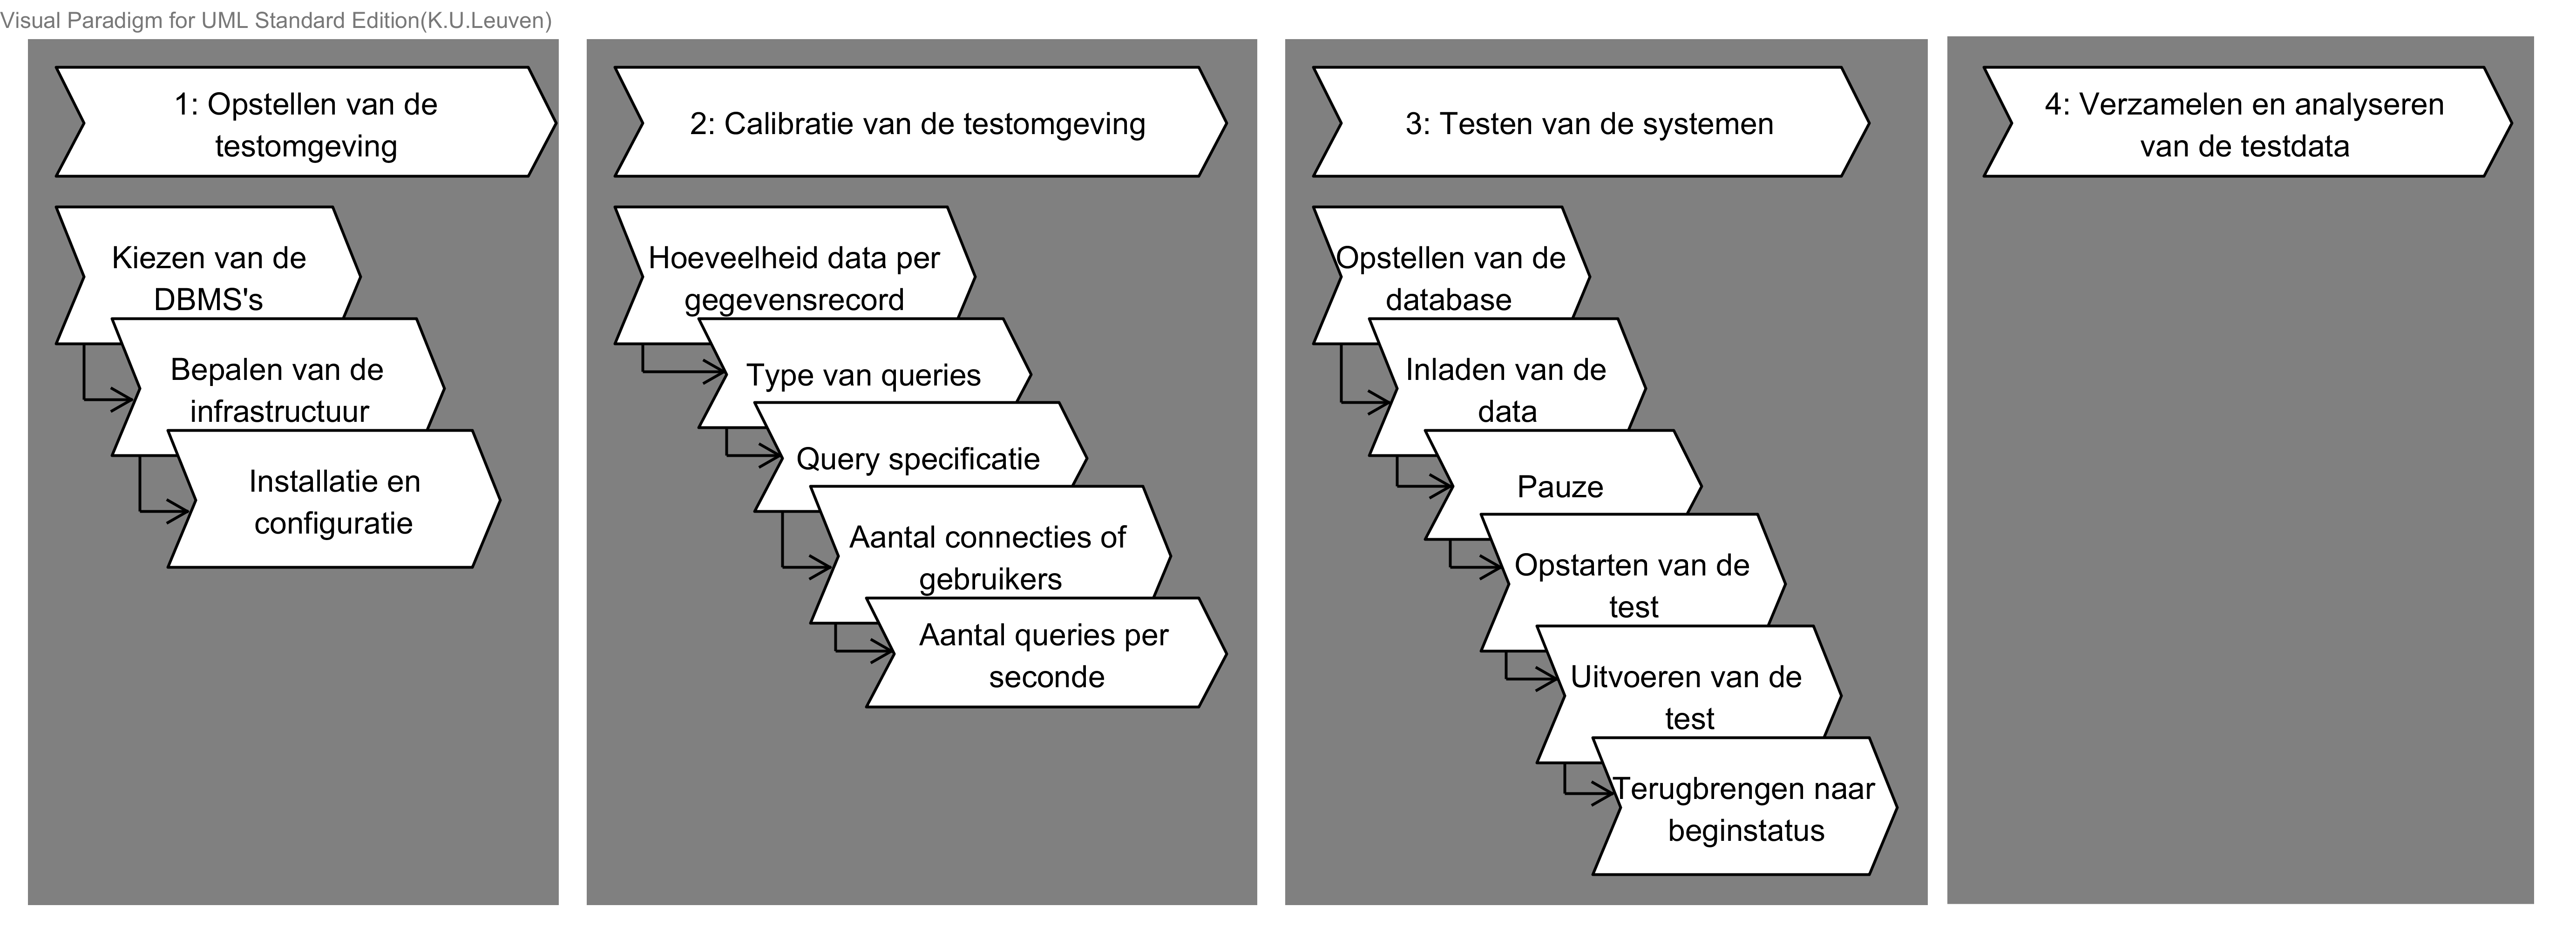
\includegraphics[width=\linewidth]{img/Test-Process-Detailed-Overview}
\caption{Overzicht testproces}
\label{fig:test-process-detailed}
\end{figure}
